% ============================================================
%  Metódy inžinierskej práce — Cvičenie 6, úloha 2 (prez.tex)
%
%  Iniciálna verzia prezentácie nášho prehľadového článku
%  "Detekcia falošných online recenzií na základe jazykových
%  a behaviorálnych príznakov" (pozri clanok.tex v koreni projektu).
%
%  Vzniklo úpravou vzorového súboru prez.tex z cvičenia c06.
%  Oproti vzoru sú pridané/upravené:
%    - názov, autor, inštitúcia a dátum našej práce,
%    - niekoľko častí (\section),
%    - slajdy s odrážkami 1. a 2. úrovne,
%    - slajd s obrázkom (diagram z UMLet) a slajd s tabuľkou,
%    - oprava kódovania (lmodern + T1 + shorthands=off), aby sa
%      dokument dal preložiť dvakrát a obsah (\tableofcontents)
%      sa korektne vygeneroval.
%
%  Preklad:  pdflatex prez.tex && pdflatex prez.tex
%  (druhý beh je potrebný kvôli obsahu a číslovaniu slajdov)
% ============================================================
\documentclass{beamer}

% ------------------------------------------------------------
%  Vzhľad (téma) — úloha 6.7: skúšame meniť \usetheme a \usecolortheme.
%  Použité je Warsaw + seahorse; ostatné možnosti sú zakomentované.
%  Systematický experiment je v súbore prez-themes.tex / build-themes.sh.
% ------------------------------------------------------------
\usetheme{Warsaw}
%\usetheme{Antibes}
%\usetheme{JuanLesPins}
%\usetheme{Goettingen}
%\usetheme{Madrid}
%\usetheme{Berlin}

\usecolortheme{seahorse}
%\usecolortheme{dolphin}
%\usecolortheme{rose}
%\usecolortheme{beaver}
% https://deic.uab.cat/~iblanes/beamer_gallery/

\setbeamercovered{transparent}

% ------------------------------------------------------------
%  Kódovanie a jazykové balíky.
%  shorthands=off je dôležité: inak sa druhý preklad (keď sa načíta
%  obsah z .toc s diakritikou) ukončí chybou "Missing $ inserted".
% ------------------------------------------------------------
\usepackage[T1]{fontenc}
\usepackage[utf8]{inputenc}
\usepackage{lmodern}                       % vektorové fonty (nie bitmapové PK)
\usepackage[slovak,shorthands=off]{babel}
\usepackage{graphicx}
\usepackage{amsmath}                       % matica a viacriadkový vzorec
\graphicspath{{../img/}{img/}}             % funguje pri preklade z cv6/ aj z koreňa
\usepackage{url}

\newcommand{\footcite}[1]{\footnote{\tiny #1}}
\newcommand{\emp}[1]{\textit{\alert{#1}}}

% ------------------------------------------------------------
%  Údaje prezentácie (úloha 6.6: názov, autor, dátum).
%  Zodpovedajú článku clanok.tex a súboru projekt-data.tex.
% ------------------------------------------------------------
\title[Detekcia falošných recenzií]{Detekcia falošných online recenzií na základe jazykových a behaviorálnych príznakov}
\subtitle{\vspace{2mm}Metódy inžinierskej práce 2026/27}
\author[Matvii Nosenko a kol.]{Matvii Nosenko, Volodymyr Nedoluha\\[1mm]Danylo Nikolenko, Rostyslav Mykytiuk}
\institute[FIIT STU]{%
	Fakulta informatiky a informačných technológií\\
	Slovenská technická univerzita v Bratislave}
\date{\footnotesize \today}

\begin{document}

% --- Titulný slajd ---
\begin{frame}[fragile=singleslide]
\titlepage
\end{frame}

% --- Motivačný slajd bez odrážok (vzor) ---
\begin{frame}[fragile=singleslide]\frametitle{O čom to je}
Online recenzie sú jedným z najvplyvnejších signálov pri nákupe tovarov
a služieb. Ich dôveryhodnosť však narúšajú falošné recenzie vytvárané
firmami, platenými recenzentmi, konkurenciou či automatizovanými nástrojmi.

Ponúkame prehľad metód detekcie a porovnávame dve hlavné skupiny príznakov:
\emph{jazykové} (čo recenzia hovorí a ako je napísaná) a \emph{behaviorálne}
(ako a kedy recenzent a platforma konajú).
\end{frame}

% --- Obsah ---
\begin{frame}[fragile=singleslide]\frametitle{Prehľad}
\tableofcontents
\end{frame}


\section{Úvod a motivácia}

\begin{frame}[fragile=singleslide]\frametitle{Prečo je to dôležité}
\begin{itemize}
\item Falošné recenzie poškodzujú spotrebiteľov a platformy
	\begin{itemize}
	\item objednané pozitívne hodnotenia zvyšujú predajnosť
	\item znevažovanie konkurencie vytvára nekalú výhodu
	\end{itemize}
\item Veľké jazykové modely (LLM) znížili náklady na tvorbu plynulého textu
	\begin{itemize}
	\item lexikálne detektory strácajú spoľahlivosť
	\item rastie význam behaviorálnych a relačných signálov
	\end{itemize}
\item Požaduje sa \emp{vysvetliteľnosť} rozhodnutia moderátora
\end{itemize}
\end{frame}

\begin{frame}[fragile=singleslide]\frametitle{Výskumné otázky}
\begin{itemize}
\item \textbf{RQ1:} Ktoré jazykové príznaky sú spojené s falošnými recenziami?
\item \textbf{RQ2:} Ktoré behaviorálne a grafové príznaky zachytávajú koordinované podvody?
\item \textbf{RQ3:} Ako tieto skupiny príznakov kombinovať?
\item \textbf{RQ4:} Ktoré problémy zostávajú otvorené v ére generatívnych modelov?
\end{itemize}
\end{frame}


\section{Súvisiace práce}

\begin{frame}[fragile=singleslide]\frametitle{Kľúčové práce v oblasti}
\begin{itemize}
\item Jindal a Liu~\footcite{\tiny Jindal \& Liu, 2008} ako prví kategorizovali recenzný spam
\item Ott a kol.~\footcite{\tiny Ott et al., 2011} vytvorili prvý štandardizovaný dataset
	\begin{itemize}
	\item n-gramy a psycholingvistické lexikóny prekonávajú ľudí
	\item klasifikátor sa učí idiosynkrázie autorov
	\end{itemize}
\item Mukherjee a kol.~\footcite{\tiny Mukherjee et al., 2013} ukázali silu behaviorálnych príznakov
\item Rayana a Akoglu~\footcite{\tiny Rayana \& Akoglu, 2015} spojili recenzie, recenzentov a produkty do jednej siete
\end{itemize}
\end{frame}


\section{Jazykové príznaky}

\begin{frame}[fragile=singleslide]\frametitle{Jazykové príznaky}
\begin{itemize}
\item \textbf{Lexikálna bohatosť:} Type-Token Ratio, dĺžka slov, slovná zásoba
	\begin{itemize}
	\item nižšia rozmanitosť sa spája s falošnými recenziami
	\item TTR treba normalizovať podľa dĺžky textu
	\end{itemize}
\item \textbf{Syntax a slovné druhy:} viac slovies, prísloviek a zámen
\item \textbf{Sémantika a sentiment:} polarita, extrémnosť hodnotenia
\item \textbf{Neurónové reprezentácie:} jemne doladené transformery (BERT)
\end{itemize}
\end{frame}

\begin{frame}[fragile=singleslide]\frametitle{Obmedzenia jazykových príznakov}
\begin{itemize}
\item Nie sú univerzálne: závisia od jazyka, domény a dĺžky recenzie
\item Slabá generalizácia a rýchle zastarávanie pri LLM-generovanom texte
\item Napriek tomu zostávajú \emp{lacné, dostupné a interpretovateľné}
\end{itemize}
\end{frame}


\section{Behaviorálne príznaky}

\begin{frame}[fragile=singleslide]\frametitle{Behaviorálne príznaky}
\begin{itemize}
\item \textbf{Recenzent:} vek účtu, počet recenzií, overený nákup, kompletnosť profilu
\item \textbf{Recenzia a produkt:} čas publikovania, duplicitný text, odchýlka od priemeru
\item \textbf{Čas:} burstiness, periodicita, synchronizácia účtov
\item \textbf{Graf a vzťahy:}
	\begin{itemize}
	\item bipartitný graf recenzent--produkt
	\item ko-recenzné skupiny a šírenie podozrenia v sieti
	\end{itemize}
\end{itemize}
\end{frame}

\begin{frame}[fragile=singleslide]\frametitle{Model dôveryhodnosti recenzenta}
Dôveryhodnosť recenzenta $u$ po $n$ recenziách modelujeme exponenciálnym
vyhladzovaním:
\begin{equation*}
T_n(u) = (1-\alpha)^n T_0(u)
+ \alpha(1-\alpha)^{n-1}\phi\bigl(r_1(u)\bigr) + \cdots
+ \alpha\phi\bigl(r_n(u)\bigr),
\end{equation*}
kde $\alpha \in (0,1)$ je miera učenia a $\phi(r_k(u)) \in \langle 0,1\rangle$
je normalizovaný signál autentickosti $k$-tej recenzie.
\end{frame}

% --- Slajd s obrázkom (úloha 6.6) ---
\begin{frame}[fragile=singleslide]\frametitle{Proces detekcie -- diagram z UMLet}
\begin{center}
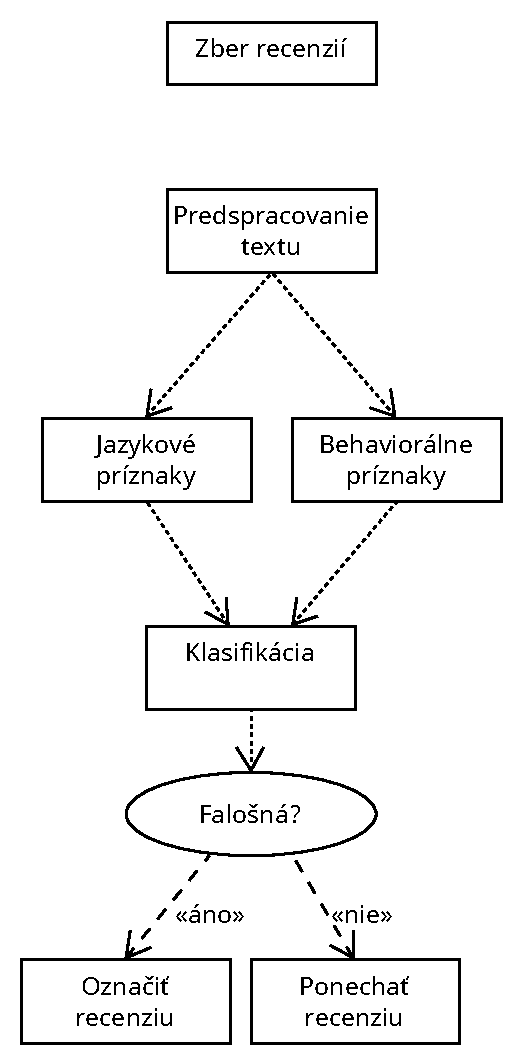
\includegraphics[width=0.72\linewidth,height=0.62\textheight,keepaspectratio]{diagram1.pdf}
\end{center}
{\tiny Diagram vytvorený v nástroji UMLet/UMLetino (\texttt{img/diagram1.pdf}).}
\end{frame}


\section{Hybridné prístupy}

\begin{frame}[fragile=singleslide]\frametitle{Hybridné a moderné prístupy}
\begin{itemize}
\item Spojenie skupín príznakov na úrovni:
	\begin{itemize}
	\item príznakov (\emph{early fusion})
	\item rozhodnutí (\emph{late fusion})
	\item spoločného modelu
	\end{itemize}
\item Osvedčené: gradientové boosting stromy, ansámble, grafové neurónové siete
\item \emp{Vysvetliteľnosť} je rovnocenný cieľ, nie doplnková funkcionalita
\item Osobitná výzva: recenzie generované LLM
\end{itemize}
\end{frame}


\section{Porovnanie a otvorené problémy}

\begin{frame}[fragile=singleslide]\frametitle{Porovnanie skupín príznakov}
\footnotesize
\begin{tabular}{@{}p{1.9cm}p{2.6cm}p{3.1cm}p{3.0cm}@{}}
\hline
\textbf{Prístup} & \textbf{Príznaky} & \textbf{Silné stránky} & \textbf{Obmedzenia} \\
\hline
Jazykový & n-gramy, TTR, sentiment & lacný, interpretovateľný & krehký voči LLM \\
Behaviorálny & frekvencia, burstiness & odolný, zachytáva koordináciu & studený štart, GDPR \\
Grafový & bipartitné grafy & odhaľuje skupiny a kampane & náročný na dáta \\
Hybridný & spojenie všetkých & najlepšia presnosť & zložitosť, preučenie \\
\hline
\end{tabular}
\vspace{2mm}
\begin{itemize}
\item Otvorené: málo slovenských/českých dát, studený štart, \emph{concept drift}
\end{itemize}
\end{frame}


\section{Navrhovaný prístup}

\begin{frame}[fragile=singleslide]\frametitle{Náš modulárny hybridný detektor}
\begin{itemize}
\item Štyri vrstvy:
	\begin{itemize}
	\item zber a anotácia dát
	\item extrakcia jazykových a behaviorálnych príznakov
	\item hybridný klasifikátor s grafovými príznakmi
	\item vrstva vysvetlenia pre moderátora
	\end{itemize}
\item Predbežné ciele: dvojjazyčný dataset (15\,000 recenzií), $\kappa \geq 0{,}7$
\item Cieľové F1: 0,80 jazykový / 0,75 behaviorálny / 0,85 hybridný model
\end{itemize}
\end{frame}


\section*{Zhodnotenie a ďalšia práca}

\begin{frame}[fragile=singleslide]\frametitle{Zhodnotenie a ďalšia práca}
\begin{itemize}
\item Jazykové príznaky sú vhodné na lacnú prvotnú filtráciu
\item Behaviorálne a grafové príznaky odhaľujú koordinované kampane
\item V ére LLM sa ťažisko presúva k hybridným riešeniam s vysvetliteľnými výstupmi
\item Ďalej: slovensko-anglický dataset a prakticky použiteľný hybridný detektor
\end{itemize}
\end{frame}

\end{document}
